%%%%%%%%%%%%%%%%%%%%%%%%%%%%%%%%%%%%%%%%%%%%
%%% CHYMISTRY
%%%%%%%%%%%%%%%%%%%%%%%%%%%%%%%%%%%%%%%%%%%%
\mysection{Chymistry}{research-chymistry}

\flavor {
    You've had your say, Potion Seller but I'll have mine. You're a rascal, you're a rascal with no respect for knights. No respect for anything... except your potions!

    \myskip

    Why respect knights... when my potions can do anything that you can?
  }


\callout {
    \mytable{Y Y} {
        \thead{\# Pips} & \thead{Coin per Pip} \\
    } {
        1-5 & 100\FE \\
        6-10 & 100\AG \\
        11+ & 100\AU
    }
}

Through the careful study of the structure and properties of certain natural substances, the Researcher is able to refine, transform and energize their quintessence to produce new and powerful essences:


\callout {\footnotesize{
\mybullet {
  \item \mybold{Elixirs:} various tonics, powders, sera, and unguents.
  \item \mybold{Laudanum:} opiatic preparations for treating \mypg{Madness!}{injury-insanity-madness}.
  \item \mybold{Malignants:} poisons, toxins, and acids.
  \item \mybold{Grenades:} petards, trombes, and bombs.
}}}

\begin{center}
  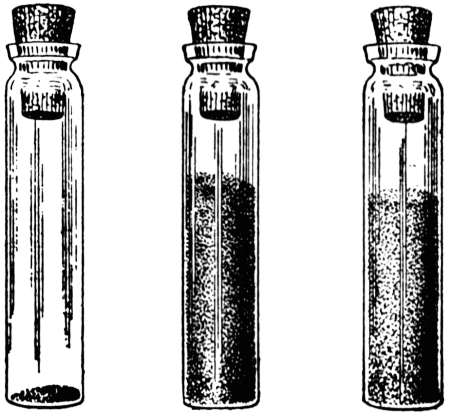
\includegraphics{research/Chymistry}
\end{center}


\cbreak

\mysubsection{Elixirs}{research-chymistry-elixirs}

Elixirs can be encountered in four different forms:

\mybold{Tonics}  are mixtures of booze, narcotics, and other things you probably don't want to know about. They must be drunk.

\mybold{Powders} can be drunk (in wine), inhaled, or smoked.  If you blow a powder in some Monster’s face, the Monster has to be able to breathe (so they don't work on undead, for example).

\mybold{Sera} need to be injected via a \mylink{Syringe}{gear-equipment}.  If the recipient is a person, they have to have a vein of some kind.  If the recipient is an object, it has to be something a needle could pierce (like an apple).

\mybold{Unguents} include oils, salves, lubricants, and pastes - basically anything you rub on things (heh heh).  They're usually super viscous and anyone will know the moment they try to drink it.  You can coat a weapon with an unguent  and "apply" it to a Monster by injuring them with the weapon (1 point of damage or more to Flesh).  If your attack misses the unguent doesn't rub off, but if you hit armor / scales / etc. without piercing Flesh, it does.  Unguents can be rubbed on someone who is who is unconscious or petrified.  The can’t be eaten as they taste shitty and will most likely be spit out, unless the eater is extremely ravenous or extremely stupid.


When created, an Elixir has \UDD{d4}. The following are the most common Elixirs:

\newpage 

\CHYMISTRY[
    Name=Al-Farabi's Calming Injection,
    Link=chymistry-al-farabis-calming-injection,
    Type=Sera,
    Pips=5,
    Time=Weeks
]

  The injected creature immediately ends \effect{Enraged}, \effect{Shaken}, or \effect{Disgusted}. If the creature is \mypg{Zoological}{monster-trait-zoological}, they become passive and docile (even removing a \mypg{Frenzied trait}{monster-trait-frenzied}).  Creatures under the effect of the Calming Injection cannot attack unless they are attacked first (if they are attacked, the effects of the injection immediately end). Unwilling creatures get a Save to negate; the effect of passivity lasts until the end of the Session.

  \CHYMISTRY[
    Name=Boyle's Sharpening Paste,
    Link=chymistry-boyles-sharpening-paste,
    Type=Unguent,
    Pips=2+,
    Time=Days
  ]

  When rubbed on the blade of a Stabbing or Chopping weapon, the weapon deals extra damage then next time it is used. The oil rubs off after a successful strike. The amount of damage depends on the number of Research Pips used:  (2) +d6; (5) +d10; (10) +d16.  


  \CHYMISTRY[
    Name=Brahe's Efficacious Sealant,
    Link=chymistry-brahes-efficacious-sealant,
    Type=Unguent,
    Pips=5,
    Time=Weeks
  ]


  A fast-drying paste that is capable of bonding stone, glass, wood, or metal (but not flesh). The Sealant lasts forever, and each use can cover an area roughly 10cm square.


\CHYMISTRY[
    Name=Chyme's Nerve Tonic,
    Link=chymistry-chymes-nerve-tonic,
    Type=Tonic,
    Pips=2+,
    Time=Days
]

This tonic grants the imbiber a +1 to all \RO and \RB tries until they take a Bivouac; for each additional 2 Research Pips you spend, you can increase the potency by +1 (up to +4 to all tries).  The imbiber cannot take a Breather, however - they are far too restless.


  \CHYMISTRY[
    Name=Cold and Drowsy Humor,
    Link=chymistry-cold-drowsy-humor,
    Type=Powder,
    Pips=5,
    Time=Days
  ]

  The imbiber stops breathing for the remainder of the Session.  They can feign death or travel underwater, are not affected by inhaled powders or gases, and are unable to speak - meaning they cannot perform certain Arcana or Vulgates.  Unwilling victims get a \SAVE{Toxins}.

\CHYMISTRY[
  Name=Cuckold's Courage,
  Link=chymistry-cuckold-courage,
  Type=Tonic,
  Pips=2,
  Time=Days
]

When quaffed, Cuckold's Courage restores 4 Grit (even over your \MAX). For every sip, the imbiber must try to \RSTRY{\VIG}; Failure gives the drinker a level of \effect{Drunk}. If you fail your \RSTRY{\VIG} when you are at \mybold{Drunk -4}, you \mypg{Overdose}{gear-narcotics-overdose}.


  \CHYMISTRY[
    Name=Dastin's Basic Talc,
    Link=chymistry-dastins-basic-talc,
    Type=Powder,
    Pips=5,
    Time=Days
  ]


  Immediately neutralizes any acid it comes in contact with. 


  \CHYMISTRY[
    Name=Faivre's Aqua Grease,
    Link=chymistry-faivres-aqua-grease,
    Type=Unguent,
    Pips=2,
    Time=Days
  ]

  A pale grease that can be rubbed on equipment to completely protect it against damage from water exposure. If rubbed on the body, allows you to swim without tiring for Hours.


\CHYMISTRY[
  Name=Fulcanelli's Clarifying Elixir,
  Link=chymistry-fulcanelli-clarifying-elixir,
  Type=Tonic,
  Pips=5,
  Time=Weeks
]

This tonic grants the drinker a bonus to resist any effects from the \mylink{Secrets of the Mind}{arcana-wizardry-secrets-alignment}. If the imbiber wouldn't normally get a Save vs. the effect, they now do; if they \mybold{do} get a Save, they can now make their try at +4.  If imbibed when the drinker is already under some effect of the Mind, the drinker immediately gives the imbiber a new Save.  This tonic immediately breaks the effects of the \mylink{Philter of von Fuchs}{chymistry-philter-von-fuchs}.




  \CHYMISTRY[
    Name=Grimm's Stuporous Preparation,
    Link=chymistry-grimms-stuporous-preparation,
    Type=Sera,
    Pips=5,
    Time=Weeks
  ]

  An injected creature of 4 \HD or less immediately becomes \effect{Slept}.

 However, if this Sera is injected into a piece of \mypg{Forbidden Fruit}{marvels-forbidden-fruit} and the fruit is ingested, the effect of the Sleep acts as a \mypg{Greater Curse}{table-greater-curses}. A \SAVE{Toxins} is allowed. This cursed slumber is permanent until the curse is fed to a \mypg{Hekaphage}{occultism-hekaphage}, or until the creator of the Forbidden Fruit either lifts the curse or is slain.  While under the curse the victim is in a state of suspended animation - they do not age, and do not need to eat or drink - but they can still be killed in the normal means (dagger through the heart, etc). Putting a creature into suspended animation will stop the effects of progressing diseases and toxins.


\CHYMISTRY[
  Name=Liebnitz Purgation,
  Link=chymistry-liebnitz-purgation,
  Type=Tonic,
  Pips=5,
  Time=Days
]


If imbibed while under the effects of an ingested Toxin, the poison is immediately vomited up and ceases to affect the victim.


\CHYMISTRY[
  Name=Philter of von Fuchs,
  Link=chymistry-philter-von-fuchs,
  Type=Tonic,
  Pips=2+,
  Time=Weeks
]

When imbibed, the drinker becomes \effect{Charmed} by the first person they see. \SAVE{Toxins} negates; otherwise, the duration depends on the number of Research Pips used:  (2) Days; (5) Weeks; (10) Months. The Philter won't affect creatures who are immune to the \mypg{Secrets of the Mind}{arcana-wizardry-secrets-alignment}.


  \CHYMISTRY[
    Name=Powdered Bezoar,
    Link=chymistry-powdered-bezoar,
    Type=Powder,
    Pips=2+,
    Time=Days
  ]


  When sprinkled on food or into a beverage, the Powdered Bezoar has a chance to neutralize the Toxin contained inside. The chance of success depends on the number of Research Pips spent: (2 Pips) 3-in-6; (4 Pips) 5-in-6; (6 Pips) Automatic Success. If a roll is needed, it is made in secret by the Arbiter.



  \CHYMISTRY[
    Name=Tesla's Silver Wash,
    Link=chymistry-teslas-silver-wash,
    Type=Unguent,
    Pips=5,
    Time=Weeks
  ]

  When applied to a 1-handed weapon, the weapon becomes permanently imbued with silver. Requires an \mypg{Ingot of silver}{settlements-money}.


  \CHYMISTRY[
    Name=Wallace's Anesthetic,
    Link=chymistry-davys-soothing-anesthetic,
    Type=Sera,
    Pips=5,
    Time=Days
  ]

  The injected creature feels any pain as pleasure until the end of the Session. Often surreptitiously given to those undergoing torture, or going under the knife for surgery. 

If the imbiber is an Adventurer, the Arbiter will roll damage against you in secret, and keep track of your Grit and Flesh for you (you keep track of your Armor). You can't ask the Arbiter how many Grit or Flesh you have left, but you can ask them how you look ("you're pretty beat up", "you're missing an arm", etc.).

If the imbiber is a Monster, treat as if the Monster had \mypg{Fanatical morale}{monster-morale}. Attacks against the Monster do +2 damage.


  \CHYMISTRY[
    Name=Wei Boyang's Alkahest,
    Link=chymistry-wei-boyangs-alkahest,
    Type=Unguent,
    Pips=5,
    Time=Weeks
  ]

  This oil will dissolve any adhesive (including Brahe's Efficacious Sealant).  Each use can cover an area roughly 10cm square.


  \CHYMISTRY[
    Name=Wordwarp,
    Link=chymistry-wordwarp,
    Type=Sera,
    Pips=5,
    Time=Weeks
  ]

  Any creature injected with this serum is affected with severe dyslexia should the fail a \SAVE{Toxins}. They are unable to read or write (including from Grimoires or Fetishes) for the rest of the Session.


  \CHYMISTRY[
    Name=Woundseal,
    Link=chymistry-woundseal,
    Type=Powder,
    Pips=2,
    Time=Days
  ]


  Sprinkling this powder on a wound immediately stops all \effect{Bleeding}.

  \begin{center}
    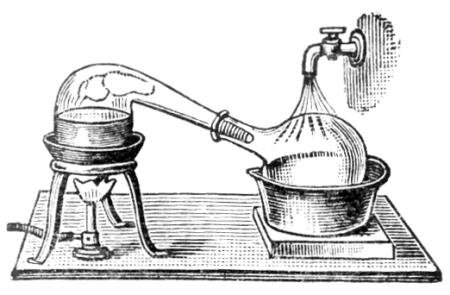
\includegraphics{research/Chymistry_2}
  \end{center}


\mysubsection{Laudanum}{research-chymistry-laudanum}

\flavor{We're all mad here. \\~ \Tilde The Cheshire cat, "Alice's Adventures in Wonderland"}

You may use your special concoctions to remove \mypg{Madness!}{injury-insanity-madness} from an unfortunate victim. Each Madness! removed requires 1 Research Pip (and 100\AG). For every Madness! removed by a \mypg{Chirurgeon}{gear-services}, multiply the costs by 5x (500\AG).



\mysubsection{Malignants}{research-chymistry-malignants}


\mybigbold{\myanchor{Acids}{malignants-acids}}

Acids can be created as liquids or powders, stored in special containers that don't react with their volatile nature (the relative fragility of these containers is at the Arbiter's discretion). Acids will dissolve flesh, stone, wood, or iron and are often used for etching, ruining locks, and pouring on people you hate.  \mybold{Each of the following effects requires 2 Research Pips}:


  \mynumlist {
    \item If the acid hits Flesh, the victim takes d4 damage for d4 Moments. If it hits Armor, the Armor \UD must be rolled at the top of every Moment.
    \item The acid can melt an area 100cm cubed of wood, metal, or stone in Minutes.
    \item When thrown on the ground, the acid will create an acrid plume of smoke that causes coughing and choking for Minutes to everything Nearby (-2 to \RO and \RB attempts).
  }

  You can sunder your Shield to negate the effect of acids thrown on you.  Acids take \mybold{Days} to make.


\mybigbold{\myanchor{Toxins}{malignants-toxins}}

\flavor{Such mortal drugs I have, but Mantua’s law / Is death to any he that utters them. \\~ \Tilde The Apothecary, "Romeo and Juliet"}

Venoms, blights, poisons, blights, and banes are grouped under \mybold{Toxins}. Like Elixirs, Toxins may be created as Tonics, Unguents, Sera, or Powders. The efficacy of the poison depends on the number of Research Pips invested:

  \mytable{Y Y Y Y} {
    \thead{Type} & \thead{\faClock[regular]} & \thead{Pips} & \thead{Downtime} \\
  } {
     Noxious & d6 & 2  & Days \\
     Deadly & d10 & 5 & Weeks \\
     Lethal & d16 & 10 & Months \\
  }

  When you are first afflicted by a Toxin, try a \SAVE{Toxins}; if you succeed, nothing happens.

  If you fail, the Arbiter should start a timer. Immediately roll the Toxin's \Duration and apply its result as damage. Every real-world minute afterwards, roll the \Duration for the Toxin and apply its result as damage. Any damage from Toxins is dealt to Grit first (wearing away your will to live) followed by Flesh. You cannot heal Grit while under the effects of a Toxin.  Note that when a Failure is finally rolled, the 1 or 2 points of damage is still dealt to your Adventurer.

 Again, note that this is a \mybold{Duration} die, meaning the effect of the poison ends if you roll a 1 or a 2, and any other roll moves the die \DCDOWN.


  \example {
Andre Preneur (Grit 4, Flesh 6) drinks a Deadly (d10) Powder dissolved in a glass of wine. Andre tries \SAVE{Toxins} - and fails, so the Arbiter starts a timer and Andre rolls a d10 and gets a 4. Andre applies 4 damage and is now at 0 Grit and 6 Flesh. His Band starts shouting excitedly over one another trying to figure out what to do. After a minute of indecision, the die moves \DCDOWN (d8) and Andre rolls again - getting a 6. Oof! Andre is now \mylink{Dying}{combat-dying}.  He will now need to make a \DEATH try every time he takes damage. The Band holds its breath as the timer marks the end of the 3rd minute ...
  }



\begin{center}
  \myimage{research/Poison}
\end{center}




\mysubsection{Grenades}{research-chymistry-grenades}

\flavor {
    Anytime I had a problem and I threw a Molotov cocktail, boom! Right away, I had a different problem. 

    ~\Tilde Jason Mendoza, The Good Place
}

Grenades are Thrown \INT weapons that have the \mypg{Splattering Attribute}{weapon-attribute-splattering}. They have different effects and strengths depending on the number of Research Pips spent. Each Grenade is a significant item and has a Burden of 1 (as they must be handled \myital{carefully}!). They take \mybold{Weeks} to make (but you can make as many as your Research Pips will allow).

\mybold{Each Grenade can only have 1 effect:}


  \mytable{Y Y} {
    \thead{Type} & \thead{Pips} \\
  } {
     Acid & 2 \\
     Bomb & 3 \\
     Chaos & 4 \\
     Concussive & 2 \\
     Explosive & 2 \\
     Fire & 2 \\     
     Flashbang  & 1  \\
     Frag & 1 \\
     Illuminating & 1  \\
     Poison Gas & 3 \\
     Screaming & 3 \\
     Smoke & 1  \\
  }

  \myhighlight{Acid}{grenade-acid}

  You may place an Acid you have created inside of the Grenade to be thrown.

  \myhighlight{Bomb}{grenade-bomb}

  Creatures Close to the point of explosion take d10 damage (\SAVE{Toxins} for half).  The bomb can have a fuse.

  \myhighlight{Chaos}{grenade-chaos}

   Creatures Close to the point of explosion must \SAVE{Toxins} or become \effect{Befuddled} and \effect{Enraged} (the source of their rage is a random Close target) for \DUR{d4}.



\myimage{research/Molotov}

  \myhighlight{Concussive}{grenade-concussive}

   Creatures Close to the point of explosion must \SAVE{Toxins} or be \effect{Knocked Out}
  \myhighlight{Explosive}{grenade-explosive}

  Creatures Close to the point of explosion take d8 damage (\SAVE{Toxins} for half).


  \myhighlight{Fire}{grenade-fire}

   Creatures Close to the point of explosion must \SAVE{Toxins} or become \effect{Enflamed}. Flammable things also catch fire (including oil).

  \myhighlight{Flashbang}{grenade-flashbang}

   Creatures Close to the point of explosion must \SAVE{Toxins} or be \effect{Stunned} for \DUR{d4}.

  \myhighlight{Frag}{grenade-frag}

  Creatures Close to the point of explosion take d6 damage (\SAVE{Toxins} for half).

\end{multicols*}
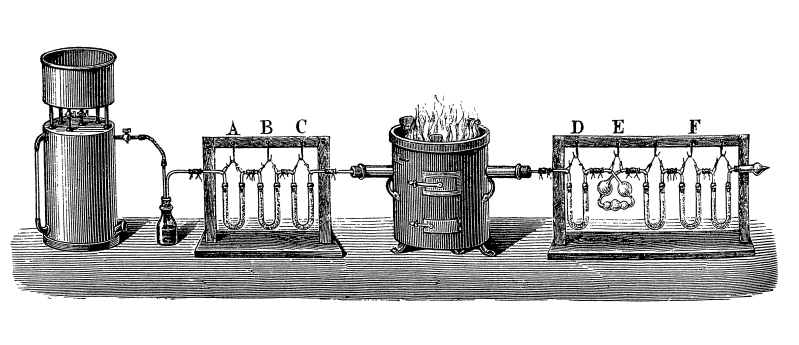
\includegraphics[width=\linewidth]{research/Lab}
\begin{multicols*}{2}

  \myhighlight{Illuminating}{grenade-illuminating}

  Creatures Close to the point of explosion must \SAVE{Toxins} or be \effect{Blinded} for \DUR{d4}.

  \myhighlight{Poison Gas}{grenade-poison}

  You may place a Toxin inside of the Grenade to be thrown.

  \myhighlight{Screaming}{grenade-screaming}

   Creatures Close to the point of explosion must \SAVE{Toxins} or become \effect{Afraid} for \DUR{d4}.

   
  \myhighlight{Smoke}{grenade-smoke}

   Everything Close to the area of impact is enveloped in smoke. The smoke acts as if a Philosopher had spoken the Secret of \mypg{Fogbank}{secrets-fogbank}, though the smoke won't move from the spot of impact. The smoke lasts for \DUR{d4}.

\newpage
